\section*{Problem 4 (15 pts)}

We learn that a deep belief network (DBN) as a generative graphical model, consists of multiple layers of latent variables with connections between the layers. 
One DBN can learn to probabilistically reconstruct its inputs and extract a deep hierarchical representation of the training data. 
DBNs can be viewed as a composition of simple, unsupervised networks such as restricted Boltzmann machines (RBMs), where each sub-network's hidden layer serves as the visible layer for the next.

In this problem, we will learn how RBMs and DBNs are trained.
Based on what you induce here, you will implement RBMs and DBNs in the following programming part.

\subsection*{Restricted Boltzmann Machine}
In the RBM, visible units are conditionally independent on hidden units and vice versa. 

\begin{center}
    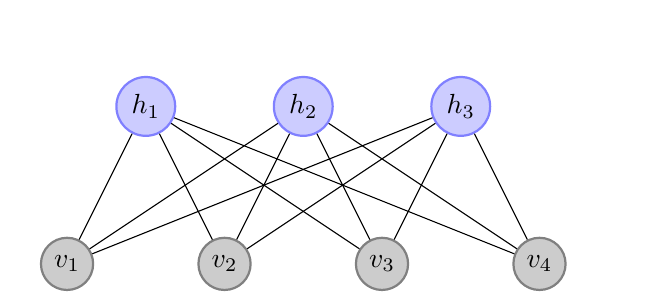
\begin{tikzpicture}
      [inner sep=1mm,
       hidden/.style={circle,draw=blue!50,fill=blue!20,thick},
       visible/.style={circle,draw=black!50,fill=black!20,thick}]
      \useasboundingbox (-0.5,0) rectangle (7,3);
      \node at (0,0) (v1) [visible] {$v_1$};
      \node at (2,0) (v2) [visible] {$v_2$};
      \node at (4,0) (v3) [visible] {$v_3$};
      \node at (6,0) (v4) [visible] {$v_4$};
      \node at (1,2) (h1) [hidden] {$h_1$};
      \node at (3,2) (h2) [hidden] {$h_2$};
      \node at (5,2) (h3) [hidden] {$h_3$};
      \foreach \x in {1,...,4}
         \foreach \y in {1,...,3}
           \draw [-] (v\x) to (h\y);
    \end{tikzpicture}
\end{center}

For a given RBM, we relate the units with the energy function as follow: 
    \[Energy(\textbf{v},\textbf{h}) = -\textbf{b}^{T}\textbf{h} - \textbf{c}^{T}\textbf{v}-\textbf{h}^{T}\textbf{W}\textbf{v}\] 
where $\textbf{b} \in \mathbb{R}^{H}, \textbf{c} \in \mathbb{R}^{V}$ are offset/bias vectors and $\textbf{W} \in \mathbb{R}^{H\times V}$ comprises the weights connecting units.

The joint probability $P(\textbf{v}, \textbf{h})$ is presented as follows:
    \[P(\textbf{v}, \textbf{h})=\frac{1}{Z}e^{-Energy(\textbf{v}, \textbf{h})}\] 
where $Z$ is the normalization term.

\subsection*{(a) Conditional probabilities $P(\textbf{v}|\textbf{h})$ and $P(\textbf{h}|\textbf{v})$ (2 pts)}
Assuming $\textbf{v}$ and $\textbf{h}$ are binary units, show $P(v_i=1 | \textbf{h})$ and $P(h_j = 1 | \textbf{v})$ are presented as follow:
\begin{align*}
    P(v_i=1|\textbf{h}) &= sigm(c_i + \textbf{h}^{T}\textbf{W}_{:,i})\\
    P(h_j=1|\textbf{v}) &= sigm(b_j + \textbf{W}_{j,:}\textbf{v})
\end{align*}
\noindent where $sigm(x) = \frac{1}{1 + e^{-x}}$.

\begin{soln}{height=\textheight}
% Put your answer here.  Please make sure you complete your answers within the given size of the box.
\end{soln}

\subsection*{(b) Free energy (3 pts)}
We obtain $P(\textbf{v})$ by marginalizing $\textbf{h}$ as follow:
    \[P(\textbf{v}) = \frac{\sum_{\textbf{h} \in \{0, 1\}^{H}} e^{-Energy(\textbf{v}, \textbf{h})}}{Z} = \frac{e^{-FreeEnergy(\textbf{v})}}{Z}\]
where $FreeEnergy(\textbf{v})$ form makes it easier to compute gradients with visible units only. 

When we rewrite the energy function as follow:
  \[Energy(\textbf{v}, \textbf{h})=-\beta(\textbf{v})-\sum_{j=1}^{H}\gamma_j(\textbf{v},h_j)\]

Show $P(\textbf{v})$ and $FreeEnergy(\textbf{v})$ could be presented as follow:
\begin{align*}
    P(\textbf{v}) &= \frac{e^{\beta(\textbf{v})}}{Z}\prod_{j=1}^{H}\sum_{h_j\in\{0, 1\}}e^{\gamma_j(\textbf{v}, h_j)} \\
    FreeEnergy(\textbf{v}) &=-\beta(\textbf{v})-\sum_{j=1}^{H}\log\sum_{h_j\in\{0, 1\}}e^{-\gamma_j(\textbf{v},h_j)} \\
    &= -\textbf{c}^{T}\textbf{v} - \sum_{j=1}^{H}\log\left(1 + e^{b_j + \textbf{W}_{j,:}\textbf{v}}\right)
\end{align*}

\begin{soln}{height=10cm}
% Put your answer here.  Please make sure you complete your answers within the given size of the box.
\end{soln}

\subsection*{(c) Log-likelihood gradient of $P(v)$ (5 pts)}
Show log-likelihood gradient of $P(v)$ could be presented as follows:
\begin{center}
    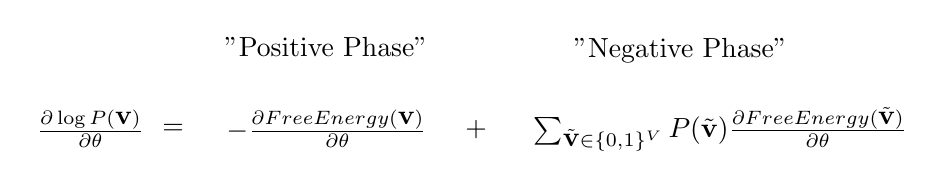
\begin{tikzpicture}[node distance=2cm]
      \node at (0,0) (a) {$\frac{\partial\log P(\textbf{v})}{\partial\theta}$};
      \node at (1.05,0) (b) {$=$};
      \node at (3,0) (c) {$-\frac{\partial FreeEnergy(\textbf{v})}{\partial\theta}$};
      \node at (4.9,0) (d) {$+$};
      \node at (8,0) (e) {$\sum_{\tilde{\textbf{v}}\in\{0,1\}^{V}}P(\tilde{\textbf{v}})\frac{\partial FreeEnergy(\tilde{\textbf{v}})}{\partial\theta}$};
      \node at (3,1.05) (f) {"Positive Phase"};
      \node at (7.5,1) (g) {"Negative Phase"};
    \end{tikzpicture}
\end{center}
Hint: present $\frac{\partial\log Z}{\partial\theta}$ in terms of $FreeEnergy(\textbf{v})$ and $P(\textbf{v})$.

\begin{soln}{height=10cm}
% Put your answer here.  Please make sure you complete your answers within the given size of the box.
\end{soln}

\subsection*{(d) Gradients with regard to each variables (5 pts)}

Show the gradients w.r.t. each variable $\textbf{W}, \textbf{b}, \textbf{c}$ could be presented as follows:
\begin{align*}
    -\frac{\partial\log P(\textbf{v})}{\partial W_{ji}} &= - P(h_j = 1|\textbf{v}) \cdot v_i + E_{\tilde{\textbf{v}}}[P(\tilde{h}_j = 1|\tilde{\textbf{v}})\cdot \tilde{v}_i] \\
    -\frac{\partial\log P(\textbf{v})}{\partial b_j} &= - P(h_j = 1 | \textbf{v}) + E_{\tilde{\textbf{v}}}[P(\tilde{h}_j = 1 | \tilde{\textbf{v}})] \\
    -\frac{\partial\log P(\textbf{v})}{\partial c_i} &= - v_i + E_{\tilde{\textbf{v}}}[\tilde{v}_i] \\
\end{align*}
Hint: use the results from (a).

\begin{soln}{height=10cm}
% Put your answer here.  Please make sure you complete your answers within the given size of the box.
\end{soln}

\subsection*{Contrastive Divergence}
In positive phase, we can compute the term with a training sample $\textbf{v}$. 
In negative phase, obtaining the expectation $E_{\tilde{\textbf{v}}}[\cdot]$ is intractable.
Contrastive Divergence replaces the expectation with a point estimate ($\tilde{\textbf{v}}, \tilde{\textbf{h}}$).
We obtain the point ($\tilde{\textbf{v}}, \tilde{\textbf{h}}$) by Gibbs sampling.
Given initial $\textbf{v}^{(0)}$, we sample $\textbf{h}^{(0)}\sim P(\textbf{h}|\textbf{v}^{(0)})$. Then we can sample $\textbf{v}^{(1)}\sim P(\textbf{v}|\textbf{h}^{(1)})$. 
After $k$ steps, we obtain $(\textbf{v}^{(k)},\textbf{h}^{(k)})$. 
As $k\rightarrow\infty$, sample $(\textbf{v}^{(k)},\textbf{h}^{(k)})$ are guaranteed to be accurate sample of $P(\textbf{v}, \textbf{h})$.
Then we can replace $E_{\tilde{\textbf{v}}}[P(\tilde{h}_j | \tilde{\textbf{v}})]$ with $P(h^{(k)}_j | \textbf{v}^{(k)})$.

\begin{center}
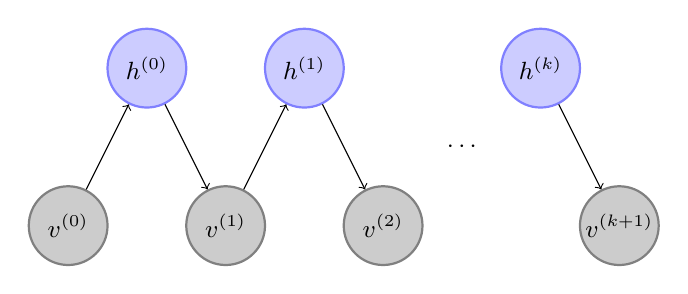
\begin{tikzpicture}
  [font=\small,
   inner sep=0pt,
   hidden/.style={circle,draw=blue!50,fill=blue!20,thick,minimum size=1cm},
   visible/.style={circle,draw=black!50,fill=black!20,thick,minimum size=1cm}]
  \node at (0,0) (v0) [visible] {$v^{(0)}$};
  \node at (1,2) (h0) [hidden]  {$h^{(0)}$};
  \node at (2,0) (v1) [visible] {$v^{(1)}$};
  \node at (3,2) (h1) [hidden]  {$h^{(1)}$};
  \node at (4,0) (v2) [visible] {$v^{(2)}$};
  \node at (6,2) (ht) [hidden]  {$h^{(k)}$};
  \node at (7,0) (vtt) [visible] {$v^{(k+1)}$};
  \draw [->] (v0) to (h0);
  \draw [->] (h0) to (v1);
  \draw [->] (v1) to (h1);
  \draw [->] (h1) to (v2);
  \draw [->] (ht) to (vtt);
  \node at (5,1) {$\cdots$};
\end{tikzpicture}
\end{center}

The initial sample in Gibbs sampling can be random values. 
Since we eventually want $P(\textbf{v})\approx P_{train}(\textbf{v})$, we start with a training example. 
Contrastive Divergence does not wait for the chain to converge. 
Only $k$-steps of Gibbs sampling is enough (so-called CD-$k$). 
$k=1$ has been shown to work surprisingly well in practice.

\subsection*{Deep Belief Network}
Top most layer is RBM. Others are directed belief networks.
\begin{center}
\begin{tikzpicture}
  \matrix (dbn)
   [matrix of math nodes,
    row sep={1.2cm,between origins},
    column sep={1.5cm,between origins},
    hidden/.style={circle,draw=blue!50,fill=blue!20,thick},
    visible/.style={circle,draw=black!50,fill=black!20,thick}]
   {
    |[hidden]|&|[hidden]|&|[hidden]|&\\
    |[hidden]|&|[hidden]|&|[hidden]|&\\
    |[hidden]|&|[hidden]|&|[hidden]|&\\
    |[visible]|&|[visible]|&|[visible]|&\\
   };
  \foreach \x [evaluate=\x as \ystart using int(\x+1)] in {2,3}
    \foreach \y in {\ystart}
      \foreach \a in {1,2,3}
        \foreach \b in {1,2,3}
          \draw [-stealth] (dbn-\x-\a) -- (dbn-\y-\b);
  \foreach \x in {1,2,3}
    \foreach \y in {1,2,3}
      \draw [-] (dbn-1-\x) -- (dbn-2-\y);
  \node at (dbn-2-3.north east) [xshift=5mm,yshift=4mm] {$\textbf{W}_3$};
  \node at (dbn-3-3.north east) [xshift=5mm,yshift=4mm] {$\textbf{W}_2$};
  \node at (dbn-4-3.north east) [xshift=5mm,yshift=4mm] {$\textbf{W}_1$};
  \node at (dbn-1-1.west) [xshift=-3mm] {$\textbf{h}^3$};
  \node at (dbn-2-1.west) [xshift=-3mm] {$\textbf{h}^2$};
  \node at (dbn-3-1.west) [xshift=-3mm] {$\textbf{h}^1$};
  \node at (dbn-4-1.west) [xshift=-3mm] {$\textbf{v}$};
  \draw [stealth-stealth] ([xshift=1cm,yshift=-1mm]dbn-1-3.east) to node [midway,xshift=12mm,yshift=1mm] {$P(\textbf{h}^2,\textbf{h}^3)$} ([xshift=1cm]dbn-2-3.east);
  \draw [-stealth] ([xshift=1cm,yshift=-1mm]dbn-2-3.east) to node [midway,xshift=12mm] {$P(\textbf{h}^1|\textbf{h}^2)$} ([xshift=1cm,yshift=1mm]dbn-3-3.east);
  \draw [stealth-] ([xshift=-1cm,yshift=-1mm]dbn-2-1.west) to node [midway,xshift=-12mm] {$Q(\textbf{h}^2|\textbf{h}^1)$} ([xshift=-1cm,yshift=1mm]dbn-3-1.west);
  \draw [-stealth] ([xshift=1cm,yshift=-1mm]dbn-3-3.east) to node [midway,xshift=12mm] {$P(\textbf{v}|\textbf{h}^1)$} ([xshift=1cm,yshift=1mm]dbn-4-3.east);
  \draw [stealth-] ([xshift=-1cm,yshift=-1mm]dbn-3-1.west) to node [midway,xshift=-12mm] {$Q(\textbf{h}^1|\textbf{v})$} ([xshift=-1cm,yshift=1mm]dbn-4-1.west);
\end{tikzpicture}
\end{center}

\textbf{DBN training}: We will use the layer-wise training algorithm. Namely, we first learn an RBM with an input layer $\textbf{v}$ and a hidden layer $\textbf{h}^{1}$, then freeze this RBM. 
We generate new training data $\textbf{h}^{1}$ by sampling $p(\textbf{h}^{1}|\textbf{v})$ for every $\textbf{v}$ in the training set (one per sample in the training set), and use this as the input to the second RBM ($\textbf{h}^{1}$ and $\textbf{h}^{2}$). 
The third RBM ($\textbf{h}^{2}$ and $\textbf{h}^{3}$) is also trained in this way.

\textbf{DBN generation}: After training a DBN, we could sample a vector $\textbf{h}^{2}$ using Gibbs sampling from the third RBM.
Given initial $\textbf{h}^{2^{(0)}}$, we sample $\textbf{h}^{3^{(0)}}\sim P(\textbf{h}^{3}|\textbf{h}^{2^{(0)}})$. 
Then we can sample $\textbf{h}^{2^{(1)}}\sim P(\textbf{h}^{2}|\textbf{h}^{3^{(0)}})$. 
After $k$ steps, we obtain $\textbf{h}^{2^{(k)}}$.
Then, using $\textbf{h}^{2^{(k)}}$, we sample lower layers, $\textbf{h}^{1}$ followed by $\textbf{v}$, using sigmoid belief networks.

\pagebreak
